% !TEX program = xelatex
\documentclass{standalone}

\usepackage{pgfplots}
\pgfplotsset{compat=newest}
\usepackage{tikz}


\begin{document}

% cone
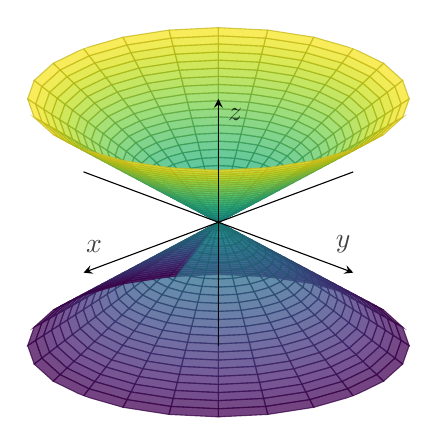
\begin{tikzpicture}
    \begin{axis}[
        axis on top,
        axis lines=center,
        set layers=default,
        xlabel={$x$}, ylabel={$y$}, zlabel={$z$},
        xtick=\empty, ytick=\empty, ztick=\empty,
        domain=0:1, y domain=0:2*pi,
        colormap/viridis,
        opacity=0.75,
        view={135}{30}
    ]

    \addplot3 [surf] ({x*cos(deg(y))}, {x*sin(deg(y))}, {x});
    \addplot3 [surf] ({x*cos(deg(y))}, {x*sin(deg(y))}, {-x});
    \end{axis}
\end{tikzpicture}

\end{document}
